
\chapter{OBSERVER BASED CONTROLS}
\label{chap:ObserverBasedControls}

Chapter \ref{chap:UNHTableSat1A} detailed how TableSat's sensor readings could be quantified and represented in terms of engineering units.  Chapter \ref{chap:SatelliteAttitudeDynamicsAndKinematics} established the state representation of the system and the chosen dynamic equations used to model it's behavior.  This chapter will focus on the estimation techniques to improve the accuracy of the state representations, and control techniques to guide the system into the desired state.

\section{Rate and Nutation Estimation Based Control with Sliding Modes}
\label{sec:RateandNutationEstimationBasedControllers}

\TODO{Add explanations}
\begin{figure}[H]
  \centerline{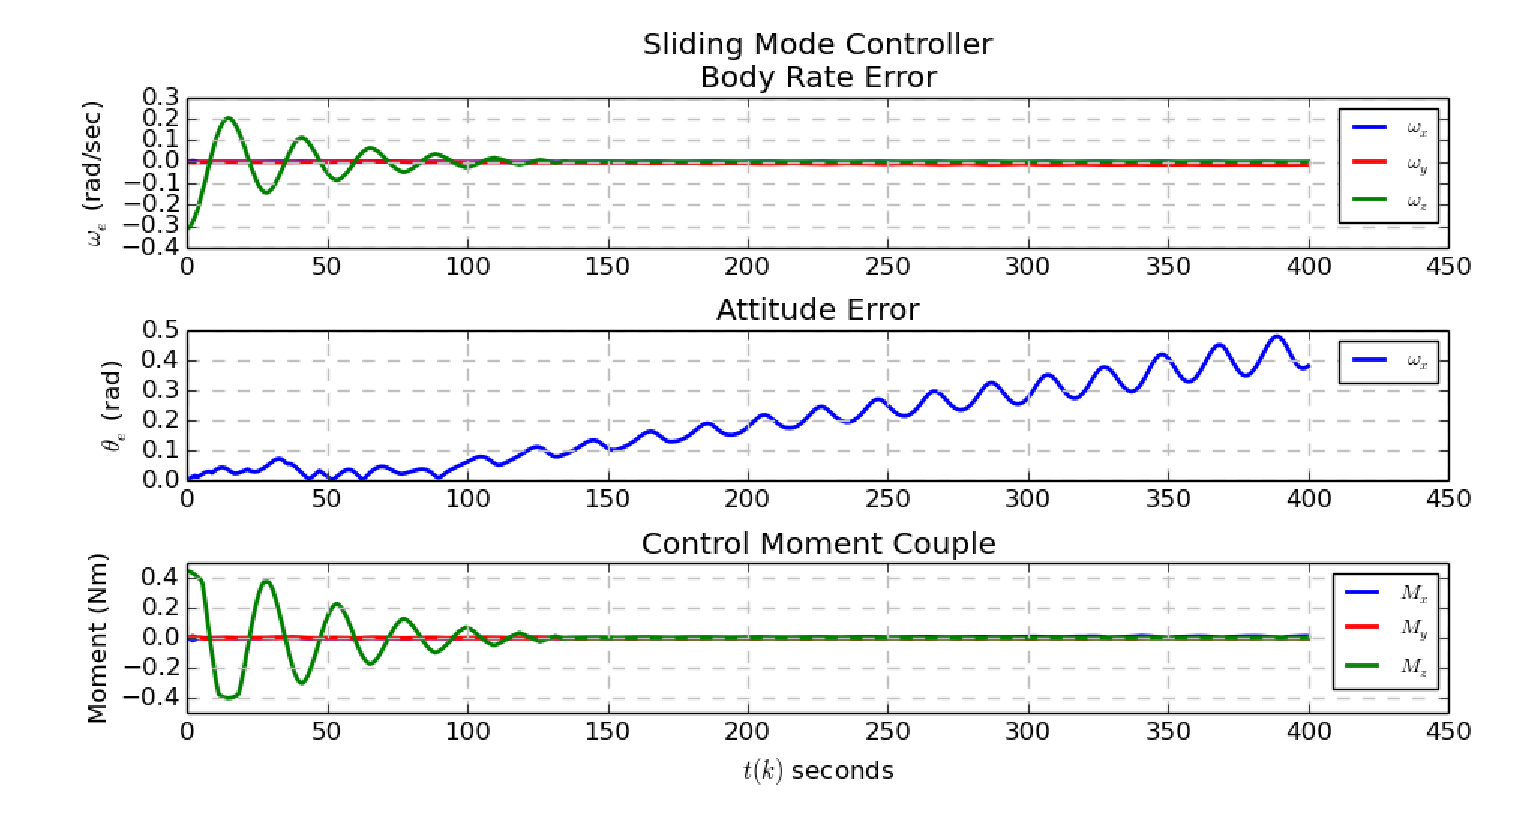
\psfig{file=figures/obc_01_smc.eps,width=6in}}
  \caption{Observer-Based Controller (SMC)}
  \label{fig:ObserverBasedControllerSMC}
\end{figure}

\begin{figure}[H]
  \centerline{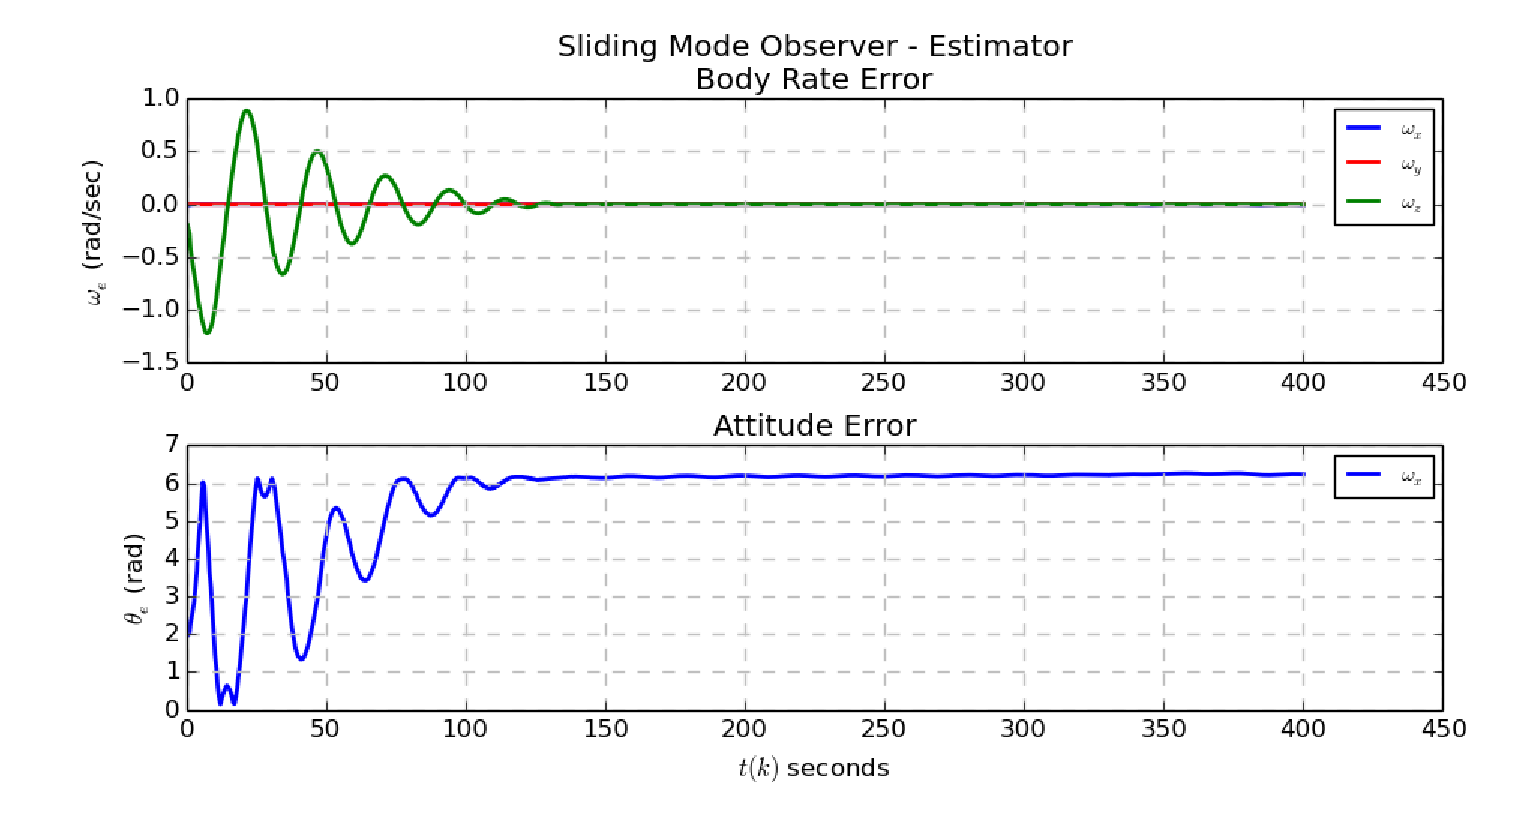
\psfig{file=figures/obc_01_smo.eps,width=6in}}
  \caption{Observer-Based Controller (SMO)}
  \label{fig:ObserverBasedControllerSMO}
\end{figure}

\begin{figure}[H]
  \centerline{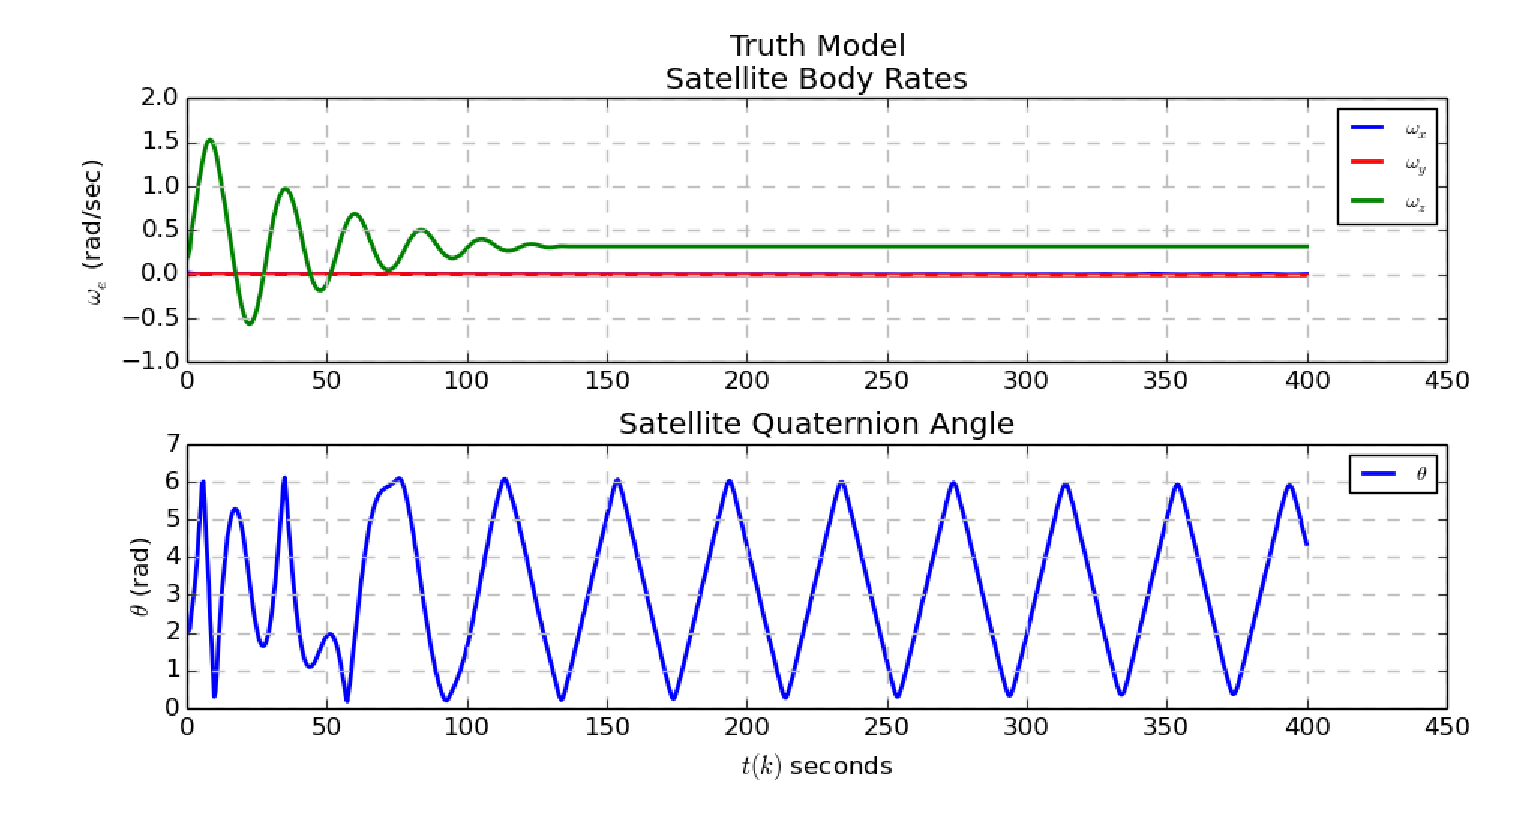
\psfig{file=figures/obc_01_truth.eps,width=6in}}
  \caption{Observer-Based Controller (Truth Model)}
  \label{fig:ObserverBasedControllerTruth}
\end{figure}


\TODO{Adding Noise}
\TODO{Unable to converge with TableSat 1A}
